\documentclass[a4paper,12pt]{article}
\usepackage[utf8]{inputenc}
\usepackage[MeX]{polski}
\usepackage{graphicx}
\hyphenation{GlobalFoundries}
\hyphenation{Giffords}

\title{Advanced Micro Devices}
\author{Patryk Kowalewski}
\begin{document}

\maketitle

\begin{abstract}\noindent Advanced Micro Devices, Inc., AMD --- amerykańskie przedsiębiorstwo produkujące elektronikę (głównie układy scalone) dla użytkowników domowych i firm. Do głównych produktów firmy należą mikroprocesory, chipsety do płyt głównych, systemy wbudowane oraz procesory graficzne dla serwerów, stacji roboczych i komputerów PC.
\end{abstract}

\begin{figure}[h]
\centering
\includegraphics[width=0.3\hsize]{amd.png}
\caption{Advanced Micro Devices}\label{AMD}
\end{figure}

\section{Historia}

Przedsiębiorstwo zostało założone 1~maja~1969 przez grupę, która odeszła z Fairchild Semiconductor, w tym Jerry’ego Sandersa, Edwina Turneya, Johna Careya, Svena Simonsena, Jacka Gifforda i trzech menedżerów z grupy Giffords: Franka Botte’a, Jima Gilesa oraz Larry’ego Stengera. Firma zaczęła produkować układy logiczne, po czym w~1975 roku rozpoczęła produkcję pamięci RAM. W tym samym roku, dzięki inżynierii odwrotnej, firma wyprodukowała klon mikroprocesora Intel~8080. W tym okresie AMD opracowywało i produkowało procesory w technologii bit slice (rodzina AMD Am2900), które były wykorzystywane w mikrokomputerach. W~1979 roku AMD zadebiutowało na nowojorskiej giełdzie. W tym samym roku rozpoczęło produkcję w nowej fabryce w Austin.
W~1991 roku firma wypuściła pierwsze procesory z serii Am386, a dwa lata później ukazały się pierwsze układy w serii Am486. W~1994 roku AMD i Compaq podpisały umowę o współpracy, dzięki czemu procesory z serii Am486 znalazły się w zestawach komputerowych tej firmy. W~2002 roku debiut miała technologia ,,Cool’n'Quiet''.


\section{Produkcja}

\begin{figure}[h]
\centering
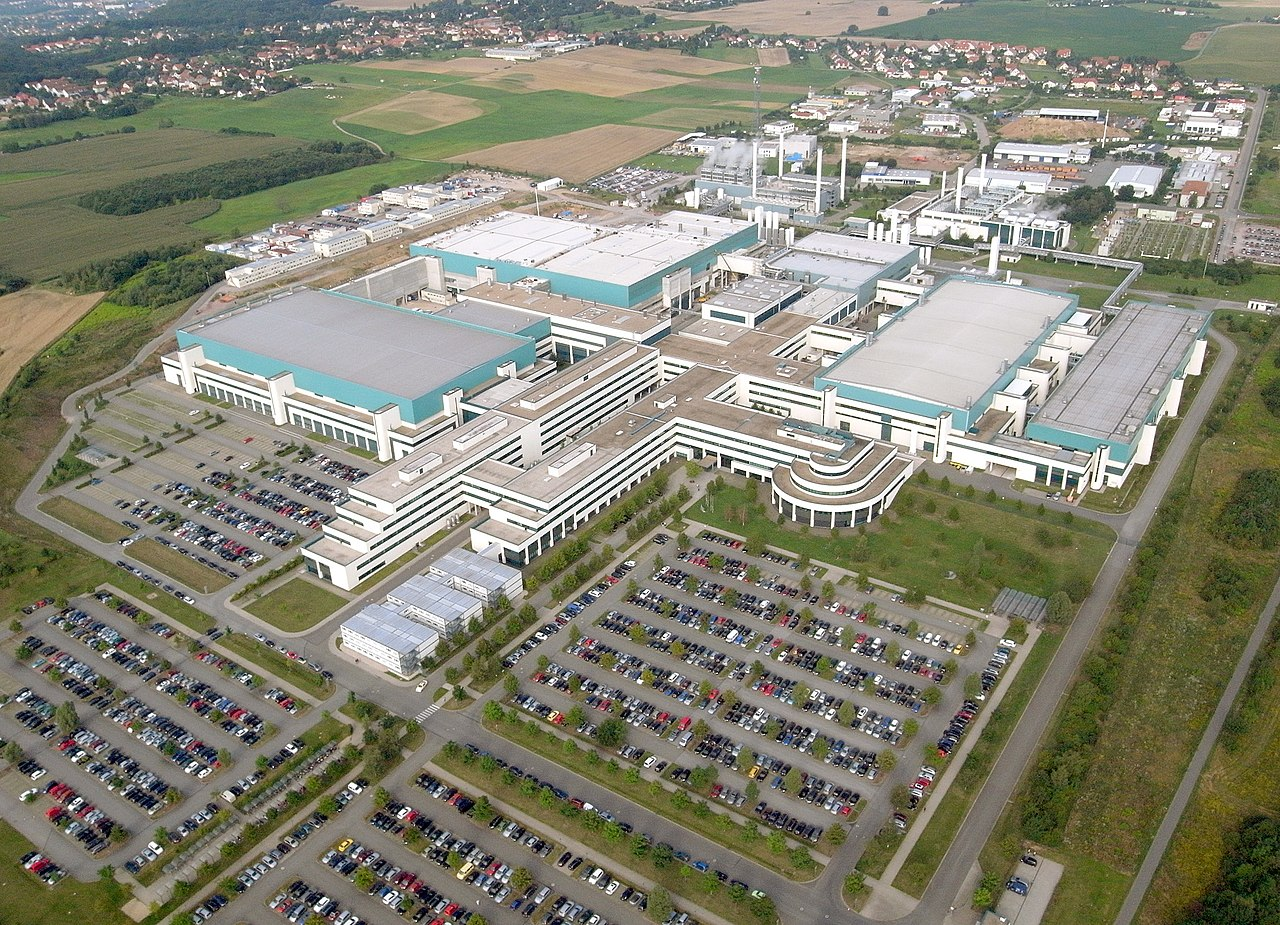
\includegraphics[width=0.5\textwidth]{fab1.jpg}
\caption{Zakład Fab 1 w Dreźnie}\label{Fab 1}
\end{figure}

Od~2009 roku za produkcję układów AMD odpowiada spółka GlobalFoundries utworzona po rozdzieleniu działu zajmującego się produkcją. Spółka posiada siedem fabryk zlokalizowanych w następujących miejscach:

\begin{table}[h]
\centering \caption{Fabryki}
\begin{tabular}{lc}
\hline
Drezno&(Fab~1)\\
Singapur&(Fab~7)\\
Hrabstwo Saratoga&(Fab~8)\\
Singapur&(Fab~2)\\
Singapur&(Fab~3/5)\\
Singapur&(Fab~3E)\\
Singapur&(Fab~6)\\
\end{tabular}
\end{table}

\footnote{Patrz Rysunek \ref{Fab 1}}



\end{document}